\documentclass[../hw4.tex]{subfiles}


\begin{document}

\subsection*{52}
Sketch the graph of the function showing all
vertical and oblique asymptotes.
\[f(x) = \frac{1+x-3x^2}{x}\]

For convenience, we rewrite $f$ as $f(x)=\frac{1}{x} + \frac{x}{x} - \frac{3x^2}{x} = \frac{1}{x} + 1 - 3x$

We will see that there is a vertical asymptote at $x=0$ by taking the limit as $x$ approaches zero from both directions.
\[\lim\limits_{x\to0} \left[ \frac{1}{x} + 1 - 3x \right]\]
As $x$ approaches zero, the magnitude of $f$ increases without bound by the term $\lim\limits_{x\to0} \frac{1}{x}$ whose limit does not exist.

We recognize that, $\lim\limits_{x\to0^-} \frac{1}{x}$ with result in increasingly large negative values while $\lim\limits_{x\to0^+}$ will produce increasingly large positive values.

For the end behavior, we take the limit as $x$ gets very large in both the positive and negative directions.
\[\lim\limits_{x\to-\infty} \left[ \frac{1}{x} + 1 - 3x \right] = 0 + 1 - \lim\limits_{x\to-\infty} 3x\]

We see that the term $\lim\limits_{x\to-\infty} 3x$ will become very large in the negative direction. Since the sign of this term is negative, $f$ will get very large as $x$ gets very large in the negative direction.
\[\lim\limits_{x\to\infty} \left[ \frac{1}{x} + 1 - 3x \right] = 0 + 1 - \lim\limits_{x\to\infty} 3x\]

Similarly, we see that the term $\lim\limits_{x\to-\infty} 3x$ will grow very large. However, since this term in negated in the sum in $f$, then $f$ will get very large in the negative direction as $x$ becomes very large in the positive direction.

We notice that these two end behaviors fall on the oblique asymptote $y=-3x$.

For the roots, we find all $x$ such that $f(x)=0$. Note that $f(x)$ is not defined at zero, so we can begin with $x\neq0$.
\begin{align*}
    \frac{1+x-3x^2}{x} &= 0 \\
    1+x-3x^2 &= 0 \\
    -3x^2+x &= -1 \\
    x^2 -\frac{x}{3} &= \frac{1}{3} \\
    {\left( x-\frac{1}{6} \right)}^2 - \frac{1}{36} &= \frac{1}{3} \\
    {\left( x-\frac{1}{6} \right)}^2 &= \frac{13}{36} \\
    x-\frac{1}{6} &= \pm \frac{\sqrt{13}}{6} \\
    x &= \frac{1 \pm \sqrt{13}}{6} \\
\end{align*}
So, the two roots are $x_1 = \frac{1-\sqrt{13}}{6}$ and $x_2 = \frac{1+\sqrt{13}}{6}$.

We differentiate $f$ with respect to $x$ to see that $f$ is decreasing for all $x \in \mathbb{R}$.
\[\frac{d}{dx} \left[ \frac{1}{x} + 1 - 3x \right] = \frac{-1}{x^2} - 3\]

Since $x^2>0$ for all $x\in\mathbb{R}$, then $f'(x)$ will always be negative.

Once more, we differentiate $f'$ to check the concavity of $f$.
\[f''(x) = \frac{d}{dx} \left[ \frac{-1}{x^2} - 3 \right] = \frac{2}{x^3}\]

For $x<0$, $f''<0$. So $f$ is concave down to the left of its asymptote at $x=0$.

For $x>0$, $f''>0$. So $f$ is concave up on the right of its vertical asymptote.

We combine these features in a sketch of the graph.


\begin{figure*}[ht]
\centering
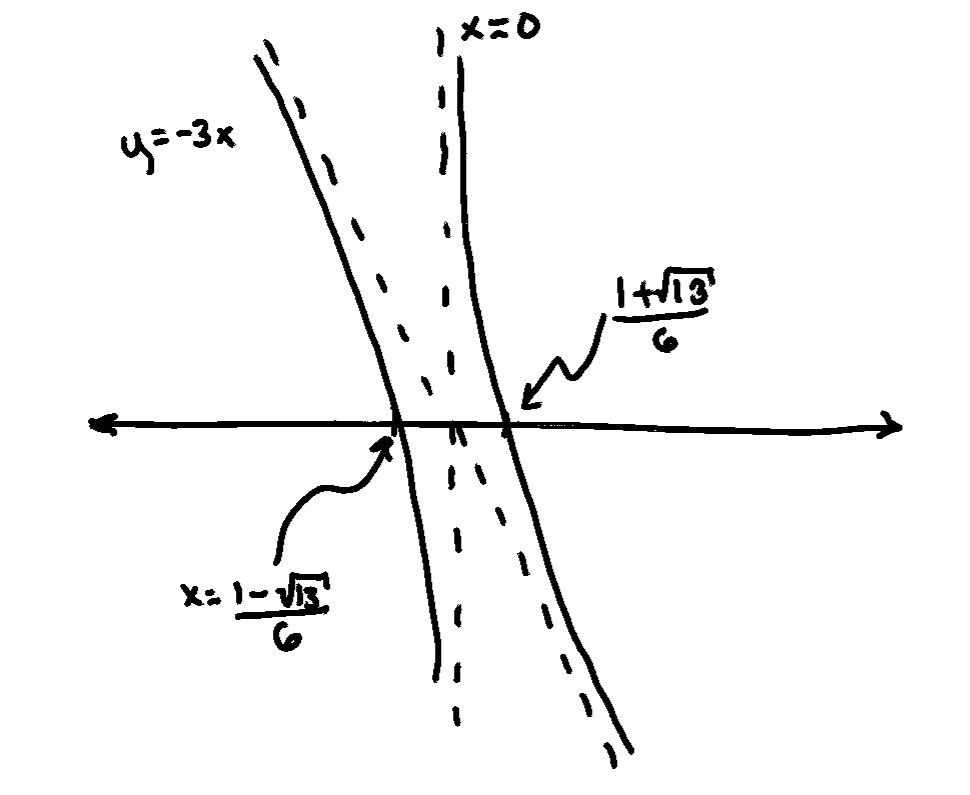
\includegraphics[width=0.5\textwidth]{figures/sketch.png}
\caption{Sketch of $f$.}
\end{figure*}

\end{document}